\section{Frontend}

Das Fronted der TeamDocument Applikation ist als React SPA entwickelt.
Einmal angemeldet kann ein Benutzer an der kollaborativen Bearbeitung des Dokumentes teilnehmen.

Folgende Interaktionen sind möglich:

\begin{itemize}
    \item Ändern des eigenen Namens
    \item Hinzufügen eines neuen Paragrafen
    \item Bearbeitung bestehender Paragrafen
    \item Sperren des Paragrafen an dem gerade gearbeitet wird (implizit)
    \item Verschieben von Paragrafen innerhalb des Dokuments
    \item Löschen eines bestehenden Paragrafen
    \item Wiederherstellen des zuletzt gelöschten Paragrafen (Hidden Feature)
\end{itemize}

Des Weiteren werden folgende Informationen auf dem UI dargestellt:

\begin{itemize}
    \item Name des ursprünglichen Authors eines Paragrafen
    \item Name des Authors welcher aktiv einen Paragrafen bearbeitet.
    \item Highlight des eigenen aktuellen Paragrafen
    \item Liste mit allen Dokumentupdates in chronologischer Reihenfolge
    \item Avatare aller aktiven Benutzer
\end{itemize}

\begin{figure}[H]
    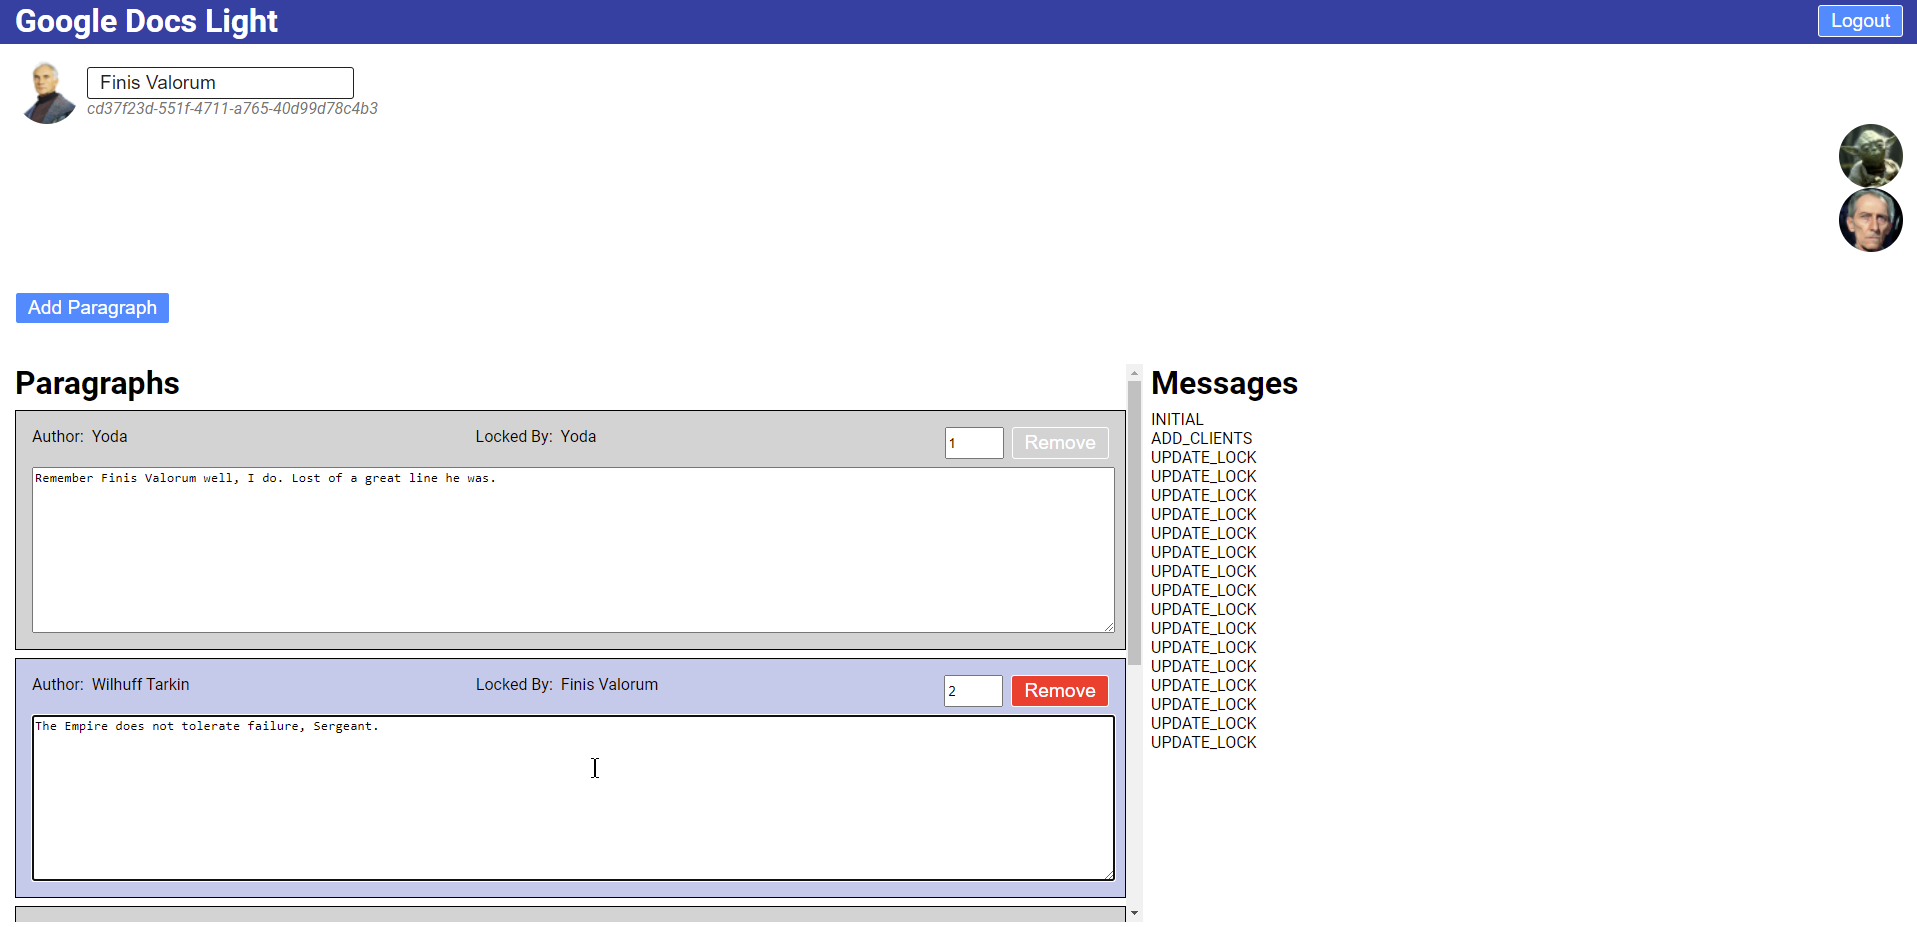
\includegraphics[width=\textwidth,keepaspectratio]{UI-blank}
    \caption{Team Document User Interface}
    \label{fig:Team Document User Interface}
\end{figure}

\subsection{Aufbau}


\subsection{Komponenten}

\begin{figure}[H]
    \centering
    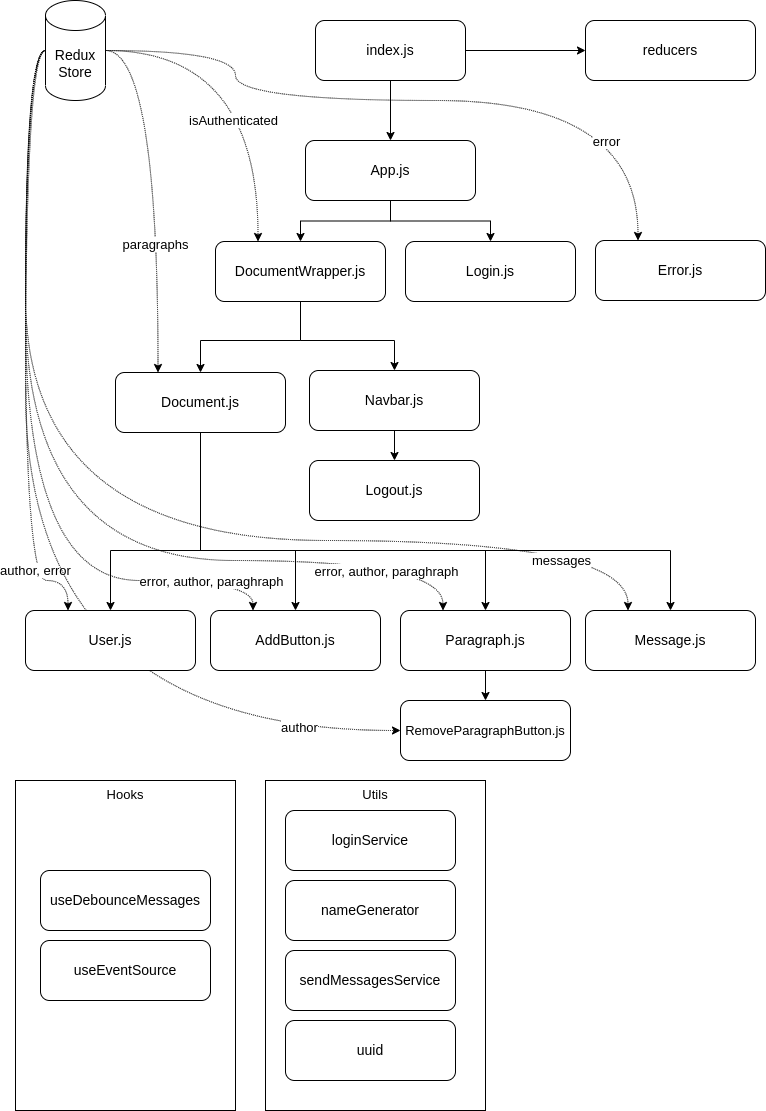
\includegraphics[width=\textwidth,keepaspectratio]{fe_structure}
    \caption{Komponenten Struktur}
    \label{fig: Fe_Structure}
\end{figure}


\begin{figure}[H]
    \centering
    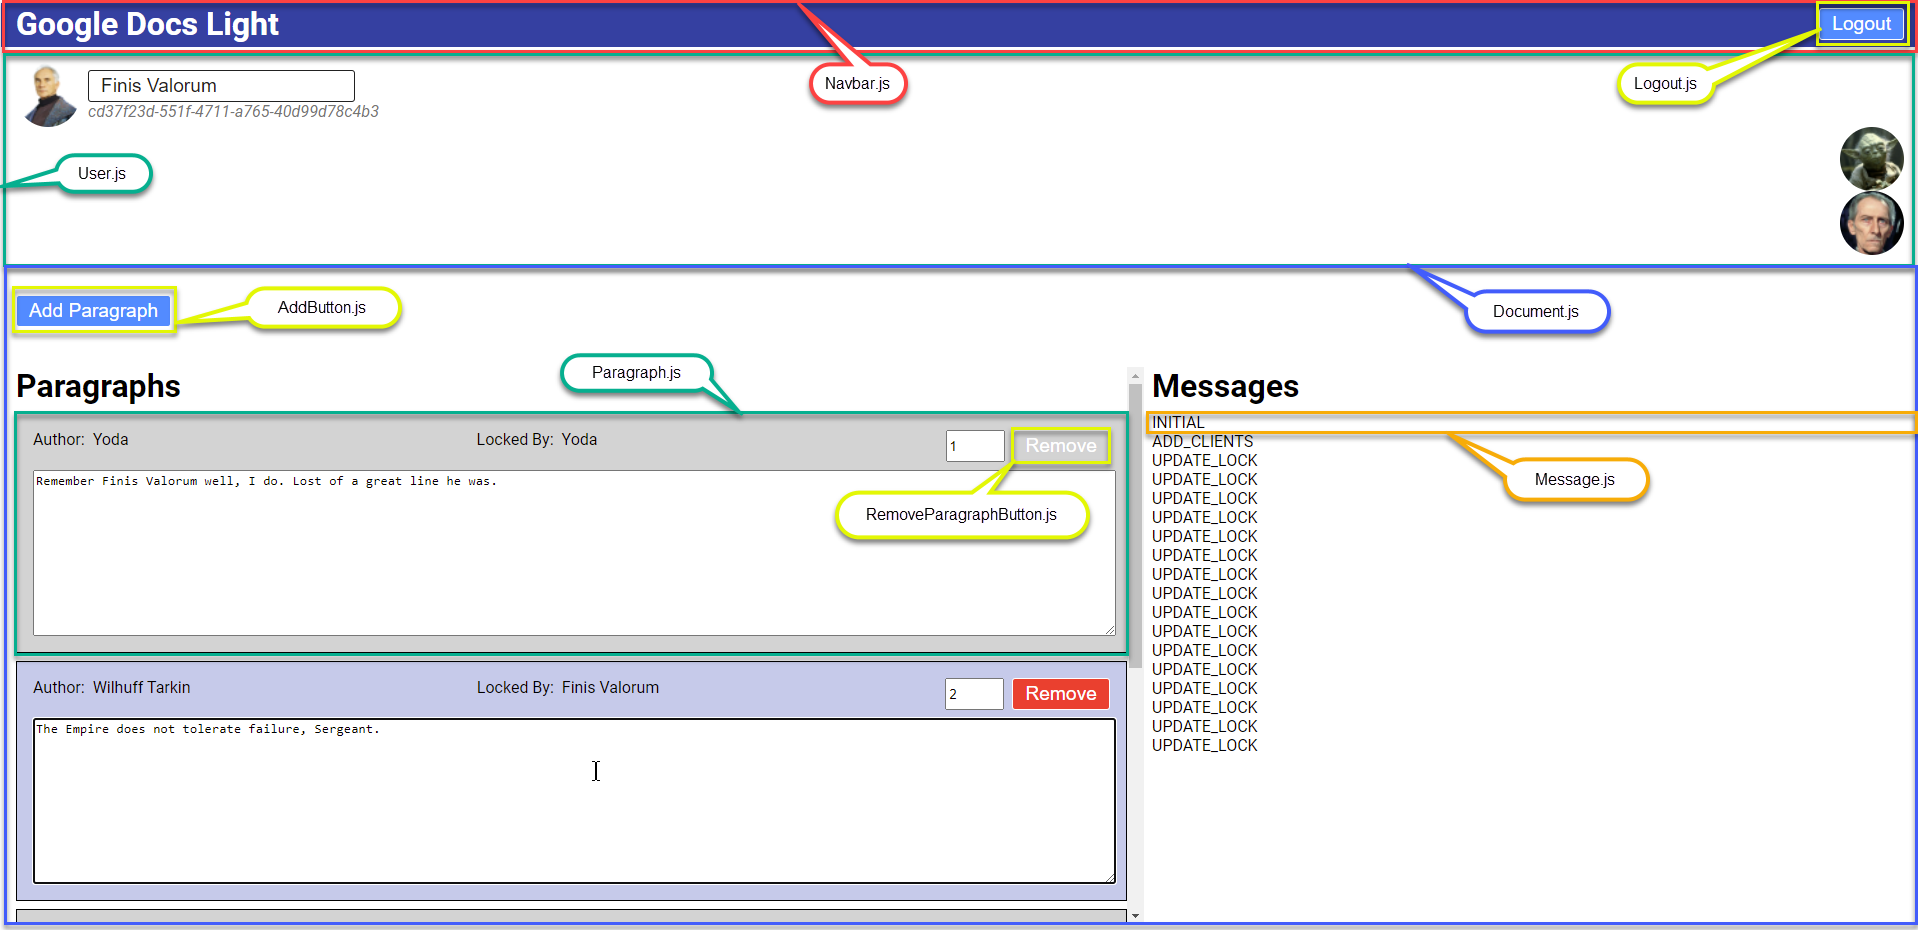
\includegraphics[width=\textwidth,keepaspectratio]{UI-components}
    \caption{UI-Components}
    \label{fig: UI-Components}
\end{figure}

\subsection{Ablaufdiagram}

\begin{figure}[H]
    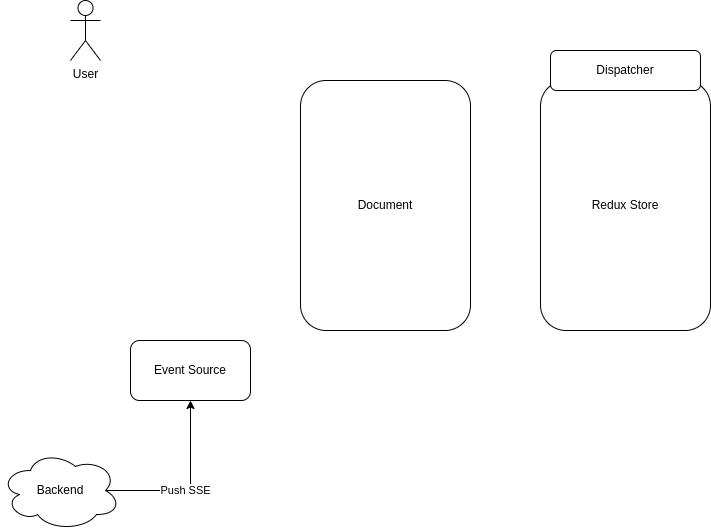
\includegraphics[width=\textwidth,keepaspectratio]{fe_dataflow}
    \caption{Datenfluss}
    \label{fig:}
\end{figure}


\subsection{State- und Konfliktmanagment}
%Redux State Verwaltung

\subsection{Fehler Behandlung}
